\input ../../SlidePreamble
\input ../../preamble


\begin{document}

{\Huge


\centerline{\bf TTIC 31230, Fundamentals of Deep Learning}
\bigskip
\centerline{David McAllester, Autumn 2020}

\vfill
\centerline{\bf Regularization: Early Stopping and Shrinkage}
\vfill
\vfill

\slide{Expectation Notation}

\begin{eqnarray*}
E_{z \sim P}\left[f(z)\right] & = & \sum_z P(z) f(z) \\
\\
\\
E_{(x,y) \sim \pop}\left[{\cal L}(x,y)\right] &  = & \frac{1}{|\mathrm{support}|}\sum_{(x,y) \in \mathrm{suppot}} \;\pop(x,y) \;{\cal L}(x,y)
\end{eqnarray*}

\vfill
Oops: the size of the support (the items with nonzero probability) is unknown.

\slide{Expectation Notation}

\vfill
Rather than sum over the support we can sample.

\vfill
Draw a sample $S = \{(x_1,y_1),\ldots,(x_N,y_N)\}$ IID from the distribution $P$.
\vfill
\begin{eqnarray*}
\hat{f}(S) & = & \frac{1}{|S|} \sum_{z\in S}\;f(z) \\
\\
\\
E_{z \sim P}\left[f(z)\right] & = & \lim_{|S| \rightarrow \infty}\;\hat{f}(S)
\end{eqnarray*}

\slide{Fitting Finite Training Data}

We take a training sample $\mathbf{Train}$ with $N$ elements.

\begin{eqnarray*}
\Phi^*(\mathbf{Train}) & = & \argmin_\Phi E_{(x,y) \sim \mathbf{Train}}\;{\cal L}_\Phi(x,y) \\
\\
& = & \argmin_\Phi \; \frac{1}{N} \sum_{(x,y)\in \mathbf{Train}}\; {\cal L}(x,y)
\end{eqnarray*}

\vfill
The training loss is typically less than the test loss.

\vfill
$$E_{(x,y) \sim \mathbf{Train}}\;{\cal L}_{\Phi^*(\mathbf{Train})}(x,y) < E_{(x,y) \sim \pop}\; {\cal L}_{\Phi^*(\mathbf{Train})}(x,y)$$

\slide{Fitting Finite Training Data}

An nth order polynomial can fit any n (pure noise) data points.


\slide{Cross Entropy Loss Vs. Task Loss}
While SGD is generally done on cross entropy loss, one often wants minimum error rate or some other leader board measure (task loss).

\vfill
The term ``loss'' often refers to cross entropy loss as opposed to task loss (leader-board metric)

\vfill
SGD typically optimizes cross-entropy loss because task loss is typically not differentiable.

\vfill
Some systems attempt to directly optimize task loss.

\vfill
But training on (cross entropy) loss is generally effective for minimizing task loss.


\slide{Early Stopping}

\centerline{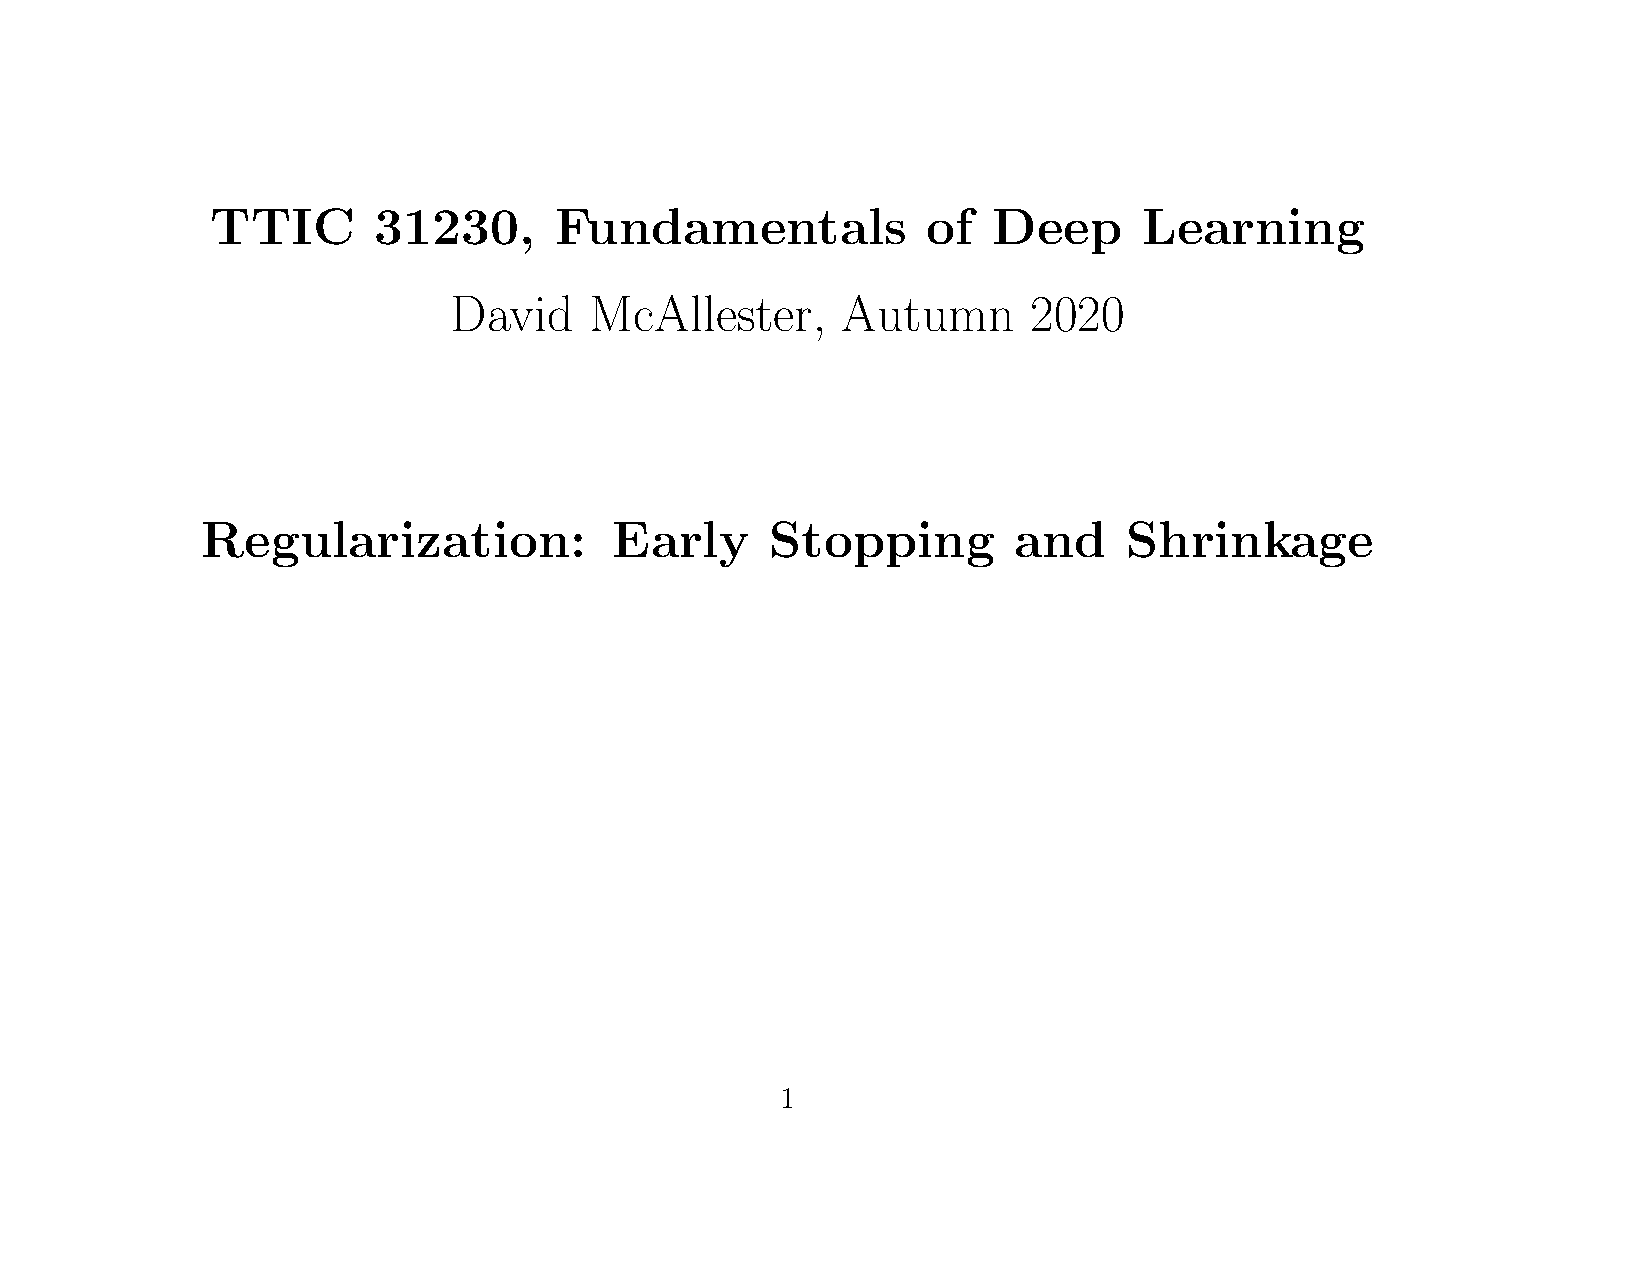
\includegraphics[height = 1.5in]{\images/Early}}

\vfill
During SGD one tracks validation loss and validation error.

\vfill
One stops training when the validation error stops improving.

\vfill
Empirically, loss reaches a minimum sooner than error.

\slide{Training Data, Validation Data and Test Data}

In general one designs algorithms and tunes hyper-parameters by training on training data and evaluating on validation data.

\vfill
But it is possible to over-fit the validation data (validation loss becomes smaller than test loss).

\vfill
Kaggle withholds test data until the final contest evaluation.


\slide{Over Confidence}

\centerline{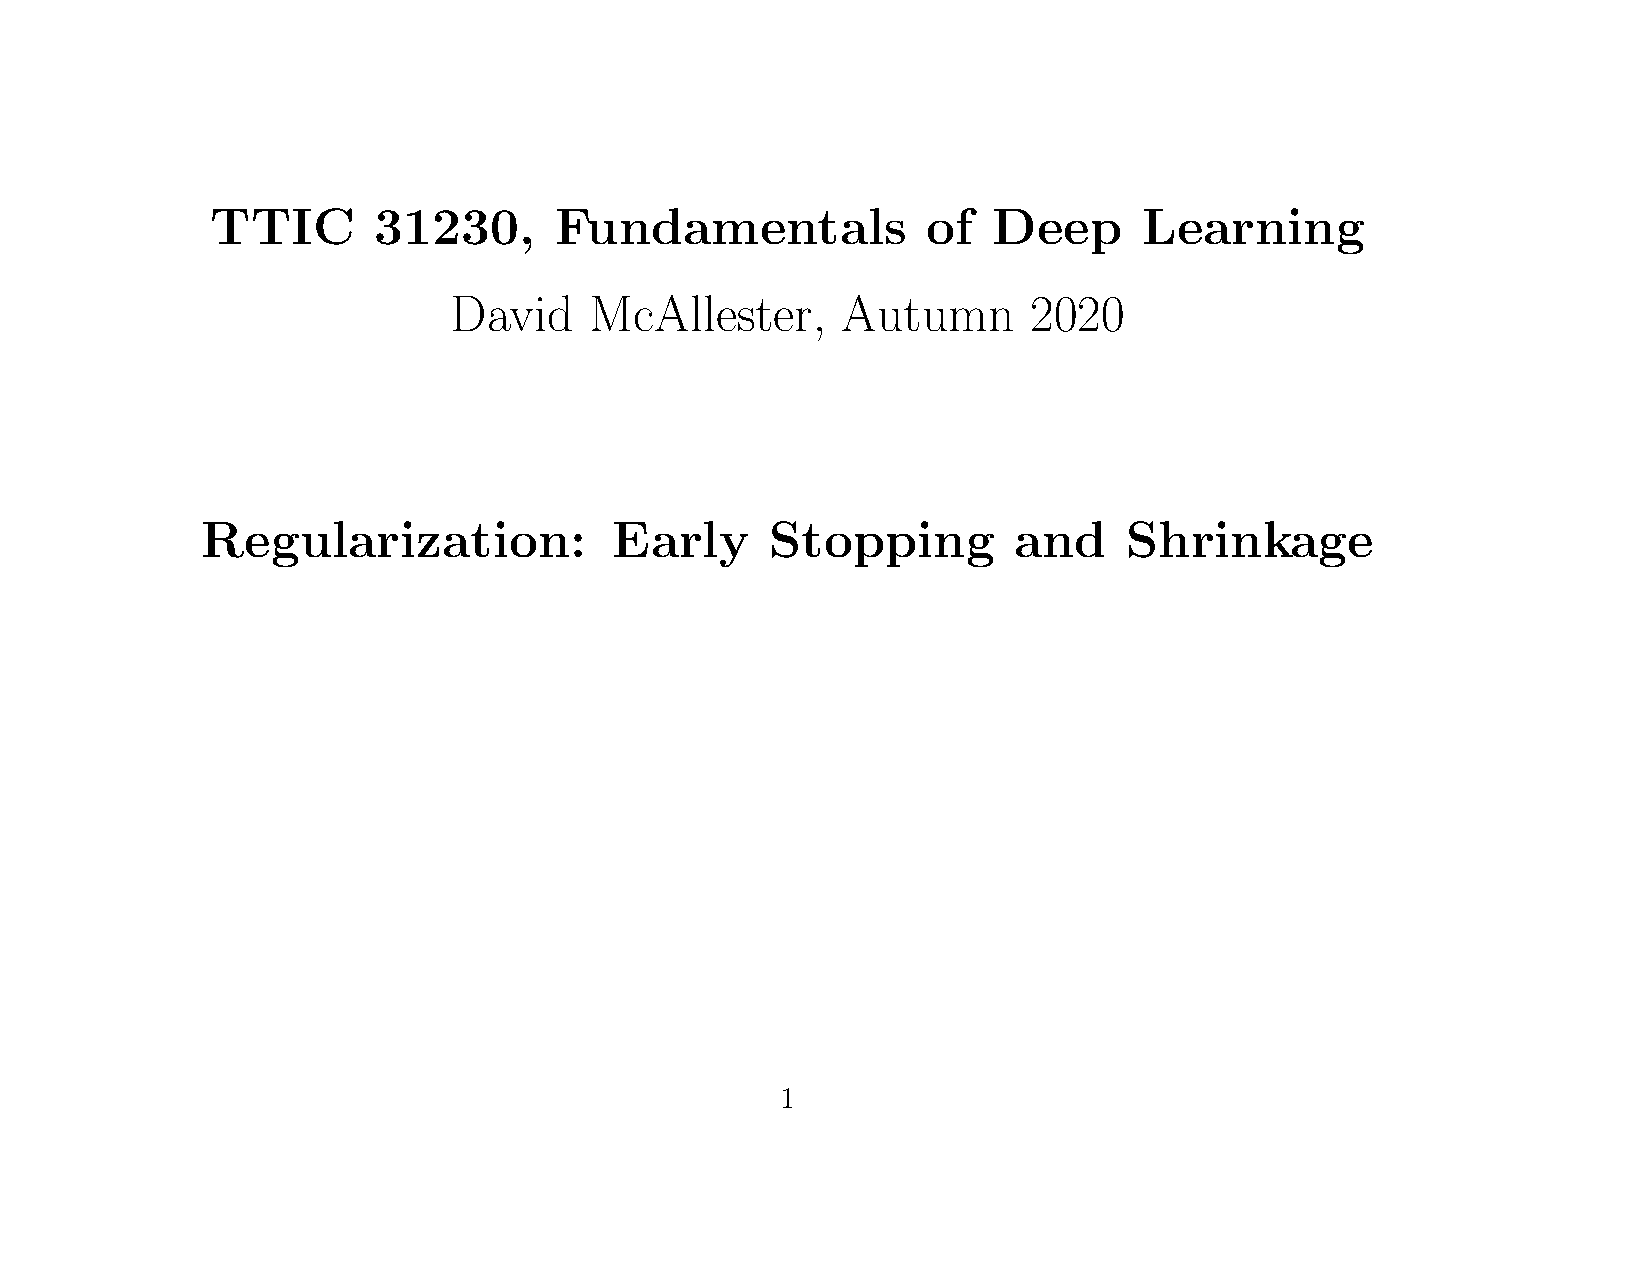
\includegraphics[height = 2in]{\images/Early}}

\vfill
Validation error is larger than training error when we stop.

\vfill
The model probabilities are tuned on training data statistics.

\vfill
The probabilities are tuned to an unrealistically low error rate and are therefore over-confident.

\vfill
This over-confidence occurs before the stopping point and damages validation loss (as opposed to validation error).

\slide{Regularization}

There is never harm in doing early stopping --- one should always do early stopping.

\vfill
Regularization is a modification to the training algorithm designed to reduce the training-validation gap and, in this way, improving overall performance.

\slide{Shrinkage: $L_2$ regularization}

We first give a Bayesian derivation. We put a prior probability on $\Phi$ and maximize the a-posteriori probability (MAP).

\vfill
{\huge
\begin{eqnarray*}
\Phi^* & = & \argmax_\Phi\;p(\Phi | \tuple{x_1,y_1},\ldots,\tuple{x_n,y_n}) \\
\\
 & = & \argmax_\Phi\;p(\Phi,\;\tuple{x_1,y_1},\ldots,\tuple{x_n,y_n}) \\
 \\
  & = & \argmax_\Phi\;p(\Phi)P(\tuple{x_1,y_1},\ldots,\tuple{x_n,y_n}\;|\;\Phi) \\
 \\
 & = & \argmax_\Phi \; p(\Phi)\;\prod_i \pop(x_i)P_\Phi(y_i|x_i) \\
 \\
  & = & \argmax_\Phi \; p(\Phi)\;\prod_i P_\Phi(y_i|x_i)
 \end{eqnarray*}
}

\slide{Shrinkage: $L_2$ Regularization}

\begin{eqnarray*}
\Phi^*   & = & \argmax_\Phi \; p(\Phi)\;\prod_i P_\Phi(y_i|x_i) \\
\\
& = & \argmin_\Phi \sum_i - \ln P_\Phi(y_i|x_i) -\ln  p(\Phi)
\end{eqnarray*}

\vfill
We now take a Gaussian prior {\color{red} $$p(\Phi) \propto \exp\left(-\frac{||\Phi||^2}{2\sigma^2}\right)$$}

\slide{Shrinkage: $L_2$ Regularization}

\begin{eqnarray*}
\Phi^* & = & \argmin_\Phi \sum_{i = 1}^n - \ln P_\Phi(y_i|x_i) + \frac{||\Phi||^2}{2\sigma^2}  \\
\\
\\
& = & \argmin_\Phi \frac{1}{N} \left(\sum_{i = 1}^n - \ln P_\Phi(y_i|x_i) + \frac{||\Phi||^2}{2\sigma^2}\right)  \\
\\
\\
& = & \argmin_\Phi \left(E_{\tuple{x,y}\sim \mathrm{Train}}\;-\ln P_\Phi(y|x)\right) + \frac{1}{2N\sigma^2} ||\Phi||^2
\end{eqnarray*}

\slide{Shrinkage: $L_2$ Regularization}

\begin{eqnarray*}
  & & \nabla_\Phi \;E_{(x,y) \sim \mathrm{Train}}\;\left({\cal L}(\Phi,x,y) + \frac{||\Phi||^2}{2N\sigma^2}\right) \\
  \\
  \\
  & = & E_{(x,y) \sim \mathrm{Train}} \;\left(g(\Phi,x,y) + \frac{\Phi}{N\sigma^2}\right)
\end{eqnarray*}

\vfill
$$\Phi_{i+1} = \Phi_i - \eta\hat{g}_i  - \frac{\eta}{N\sigma^2}\Phi_i$$

\vfill
The last term in the update equation is called ``shrinkage''.

\slide{Robust Shrinkage}

The PyTorch parameters are $\eta$ and $\gamma$:

$${\color{red} \Phi_{i+1}} = \Phi_i - \eta\hat{g} - \frac{\eta}{N\sigma^2}\Phi_i\;\;\;\; = {\color{red} \Phi_i - \eta\hat{g} - \gamma\Phi_i}$$

\vfill
To make SGD with shrinkage robust to changes in training size, batch size, learning rate (temperature) and momentum we can use

\vfill
{\color{red} $$\eta = (1-\mu)B\eta_0\;\;\;\;\;\;\;\;\;\gamma = \frac{\eta}{N_{\mathrm{Train}}\sigma^2}$$}

\vfill
where $\eta_0$ is the robust temperature parameter and $\sigma^2$ is the robust shrinkage parameter.

\slide{END}

}
\end{document}
